\section{Introduction to Systems of Differential Equations}

\noindent
Many physical situations are modelled by systems of $n$ differential equations in $n$ unknown
functions, where $n\ge2$. The next three examples illustrate physical problems that lead to systems
of differential equations. In these examples and throughout this chapter we'll denote the
independent variable by $t$.

\begin{example}
  \label{example:10.1.1} \rm Tanks $T_{1}$ and $T_{2}$ contain 100 gallons and 300 gallons of salt
  solutions, respectively. Salt solutions are simultaneously added to both tanks from external
  sources, pumped from each tank to the other, and drained from both tanks
  (Figure~\ref{figure:10.1.1}). A solution with $1$ pound of salt per gallon is pumped into $T_{1}$
  from an external source at $5$~gal/min, and a solution with $2$ pounds of salt per gallon is
  pumped into $T_{2}$ from an external source at $4$~gal/min. The solution from $T_{1}$ is pumped
  into $T_{2}$ at 2 gal/min, and the solution from $T_{2}$ is pumped into $T_{1}$ at $3$ gal/min.
  $T_{1}$ is drained at $6$~gal/min and $T_{2}$ is drained at 3~gal/min. Let $Q_{1}(t)$ and
  $Q_{2}(t)$ be the number of pounds of salt in $T_{1}$ and $T_{2}$, respectively, at time $t>0$.
  Derive a system of differential equations for $Q_{1}$ and $Q_{2}$. Assume that both mixtures are
  well stirred.
\end{example}

\begin{figure}[H]
  \centering
  \color{blue}
  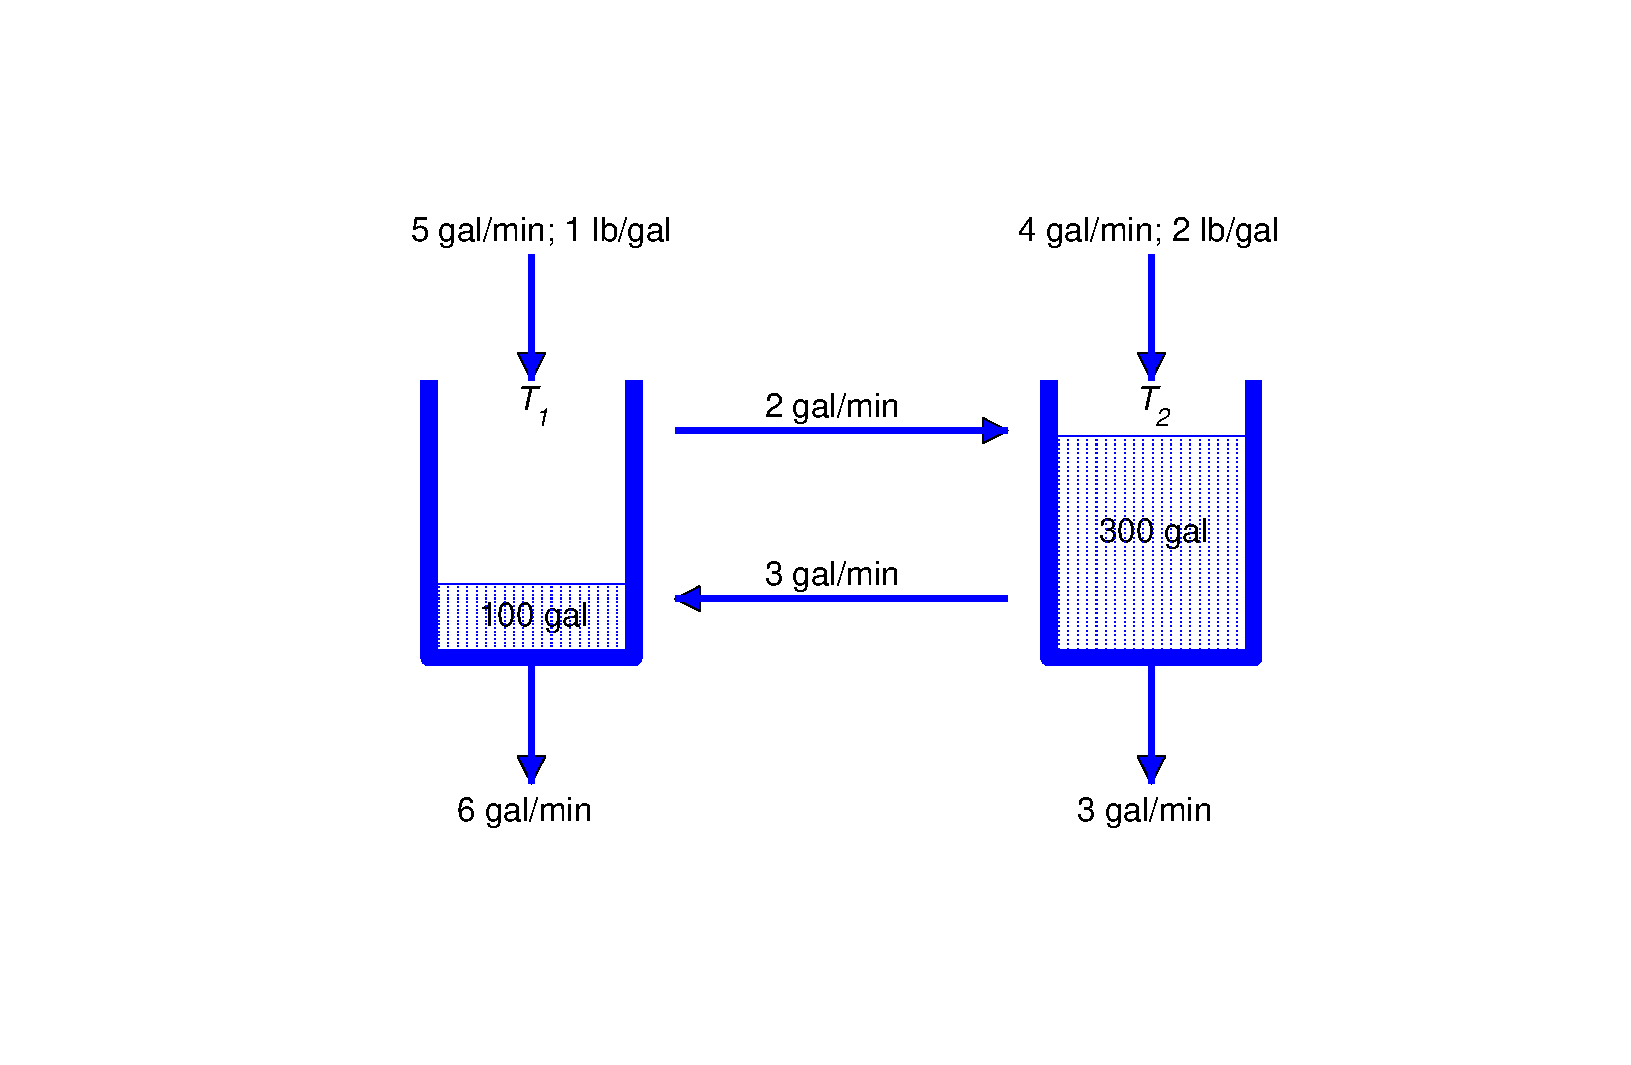
\includegraphics[bb=-78 148 689 643, width=5.67in, height=3.66in, keepaspectratio]{fig100101}
  \caption{}
  \label{figure:10.1.1}
\end{figure}

\solution As in Section~4.2, let {\color{blue}\it rate in\/} and {\color{blue}\it rate out\/} denote
the rates (lb/min) at which salt enters and leaves a tank; thus,
\begin{eqnarray*}
  Q_{1}' & = & (\mbox{rate in})_{1}-(\mbox{rate out})_{1}, \\[2\jot]
  Q_{2}' & = & (\mbox{rate in})_{2}-(\mbox{rate out})_{2}.
\end{eqnarray*}
Note that the volumes of the solutions in $T_{1}$ and $T_{2}$ remain constant at 100~gallons and
300~gallons, respectively.

$T_{1}$ receives salt from the external source at the rate of
\[
  \mbox{(1 lb/gal) }\times\mbox{ (5~gal/min)}=\mbox{ 5 lb/min},
\]
and from $T_{2}$ at the rate of
\[
  \mbox{(lb/gal in }T_{2})\times\mbox{ (3~gal/min) }=\frac{1}{300}Q_{2}\times3\\[2\jot]=\frac{1}{100}Q_{2}\mbox{ lb/min}.
\]
Therefore
\begin{equation}
  \label{eq:10.1.1}\mbox{(rate in)}_{1}=5+\frac{1}{100}Q_{2}.
\end{equation}
Solution leaves $T_{1}$ at the rate of 8~gal/min, since 6~gal/min are drained and 2~gal/min are
pumped to $T_{2}$; hence,
\begin{equation}
  \label{eq:10.1.2}(\mbox{rate out})_{1}=(\mbox{ lb/gal in T}_{1})\times\mbox{(8~gal/min) }=\frac{1}{100}Q_{1}\times8=\frac{2}{25}Q_{1}.
\end{equation}
Eqns.~\eqref{eq:10.1.1} and \eqref{eq:10.1.2} imply that
\begin{equation}
  \label{eq:10.1.3}Q_{1}'=5+\frac{1}{100}Q_{2}-\frac{2}{25}Q_{1}.
\end{equation}

$T_{2}$ receives salt from the external source at the rate of
\[
  \mbox{(2 lb/gal) }\times\mbox{ (4~gal/min)}=\mbox{ 8 lb/min},
\]
and from $T_{1}$ at the rate of
\[
  \mbox{(lb/gal in }T_{1})\times\mbox{ (2~gal/min) }=\frac{1}{100}Q_{1}\times2\\[2\jot]=\frac{1}{50}Q_{1}\mbox{ lb/min}.
\]
Therefore
\begin{equation}
  \label{eq:10.1.4}\mbox{(rate in)}_{2}=8+\frac{1}{50}Q_{1}.
\end{equation}
Solution leaves $T_{2}$ at the rate of $6$~gal/min, since $3$~gal/min are drained and $3$~gal/min
are pumped to $T_{1}$; hence,
\begin{equation}
  \label{eq:10.1.5}(\mbox{rate out})_{2}=(\mbox{ lb/gal in T}_{2})\times\mbox{(6~gal/min) }=\frac{1}{300}Q_{2}\times6=\frac{1}{50}Q_{2}.
\end{equation}
Eqns.~\eqref{eq:10.1.4} and \eqref{eq:10.1.5} imply that
\begin{equation}
  \label{eq:10.1.6}Q_{2}'=8+\frac{1}{50}Q_{1}-\frac{1}{50}Q_{2}.
\end{equation}

We say that \eqref{eq:10.1.3} and \eqref{eq:10.1.6} form a {\color{blue}\it system of two first
order equations in two unknowns\/}, and write them together as
\begin{eqnarray*}
  Q_{1}' & = & \dst{5-\frac{2}{25}Q_{1}+\frac{1}{100}Q_{2}} \\
  Q_{2}' & = & \dst{8+\frac{1}{50}Q_{1}-\frac{1}{50}Q_{2}}.\quad\bbox
\end{eqnarray*}

\begin{example}
  \label{example:10.1.2} \rm A mass $m_{1}$ is suspended from a rigid support on a spring $S_{1}$
  and a second mass $m_{2}$ is suspended from the first on a spring $S_{2}$
  (Figure~\ref{figure:10.1.2}). The springs obey Hooke's law, with spring constants $k_{1}$ and
  $k_{2}$. Internal friction causes the springs to exert damping forces proportional to the rates of
  change of their lengths, with damping constants $c_{1}$ and $c_{2}$. Let $y_{1}=y_{1}(t)$ and
  $y_{2}=y_{2}(t)$ be the displacements of the two masses from their equilibrium positions at time
  $t$, measured positive upward. Derive a system of differential equations for $y_{1}$ and $y_{2}$,
  assuming that the masses of the springs are negligible and that vertical external forces $F_{1}$
  and $F_{2}$ also act on the objects.
\end{example}

\solution In equilibrium, $S_{1}$ supports both $m_{1}$ and $m_{2}$ and $S_{2}$ supports only
$m_{2}$. Therefore, if $\Delta\ell_{1}$ and $\Delta\ell_{2}$ are the elongations of the springs in
equilibrium then
\begin{equation}
  \label{eq:10.1.7}(m_{1}+m_{2})g=k_{1}\Delta\ell_{1}\quad\mbox{ and }\quad m_{2}g=k_{2}\Delta\ell_{2}.
\end{equation}

\begin{figure}[tbp]
  \centering
  \color{blue}
  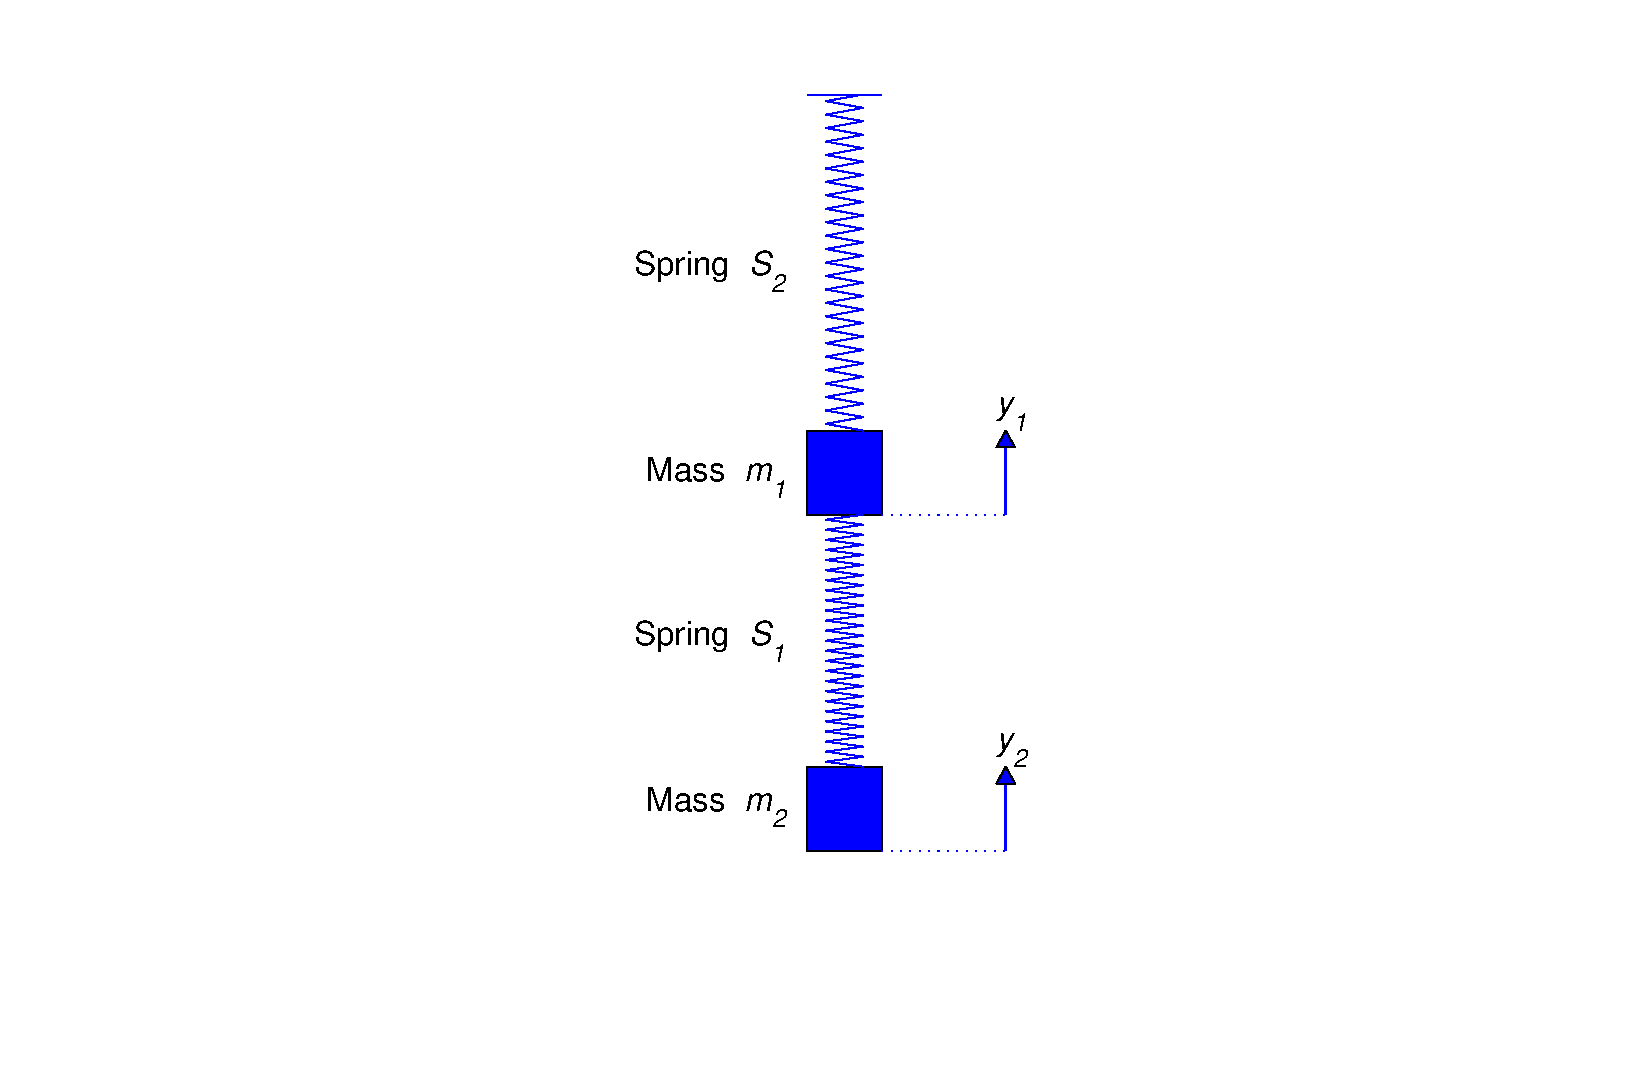
\includegraphics[bb=-78 148 689 643, width=5.67in, height=3.66in, keepaspectratio]{fig100102}
  \caption{}
  \label{figure:10.1.2}
\end{figure}

Let $H_{1}$ be the Hooke's law force acting on $m_{1}$, and let $D_{1}$ be the damping force on
$m_{1}$. Similarly, let $H_{2}$ and $D_{2}$ be the Hooke's law and damping forces acting on $m_{2}$.
According to Newton's second law of motion,
\begin{equation}
  \label{eq:10.1.8}
  \begin{array}{ccl}
    m_{1}y_{1}''=-m_{1}g+H_{1}+D_{1}+F_{1}, \\[1\jot]
    m_{2}y_{2}''=-m_{2}g+H_{2}+D_{2}+F_{2}.
  \end{array}
\end{equation}
When the displacements are $y_{1}$ and $y_{2}$, the change in length of $S_{1}$ is
$-y_{1}+\Delta\ell_{1}$ and the change in length of $S_{2}$ is $-y_{2}+y_{1}+\Delta\ell_{2}$. Both
springs exert Hooke's law forces on $m_{1}$, while only $S_{2}$ exerts a Hooke's law force on
$m_{2}$. These forces are in directions that tend to restore the springs to their natural lengths.
Therefore
\begin{equation}
  \label{eq:10.1.9}H_{1}=k_{1}(-y_{1}+\Delta\ell_{1})-k_{2}(-y_{2}+y_{1}+\Delta\ell_{2})\quad\mbox{ and }\quad H_{2}=k_{2}(-y_{2}+y_{1}+\Delta\ell_{2}).
\end{equation}
When the velocities are $y_{1}'$ and $y_{2}'$, $S_{1}$ and $S_{2}$ are changing length at the rates
$-y_{1}'$ and $-y_{2}'+y_{1}'$, respectively. Both springs exert damping forces on $m_{1}$, while
only $S_{2}$ exerts a damping force on $m_{2}$. Since the force due to damping exerted by a spring
is proportional to the rate of change of length of the spring and in a direction that opposes the
change, it follows that
\begin{equation}
  \label{eq:10.1.10}D_{1}=-c_{1}y_{1}'+c_{2}(y_{2}'-y_{1}')\quad\mbox{ and }\quad D_{2}=-c_{2}(y_{2}'-y_{1}').
\end{equation}

From \eqref{eq:10.1.8}, \eqref{eq:10.1.9}, and \eqref{eq:10.1.10},
\begin{equation}
  \label{eq:10.1.11}
  \begin{array}{ccl}
    m_{1}y_{1}'' & =       & -m_{1}g+k_{1}(-y_{1}+\Delta\ell_{1})-k_{2}(-y_{2}+y_{1}+\Delta\ell_{2})         \\[1\jot]
                 & \mbox{} & -c_{1}y_{1}'+c_{2}(y_{2}'-y_{1}')+F_{1}                                         \\[1\jot]
                 & =       & -(m_{1}g-k_{1}\Delta\ell_{1}+k_{2}\Delta\ell_{2})-k_{1}y_{1}+k_{2}(y_{2}-y_{1}) \\[1\jot]
                 & \mbox{} & -c_{1}y_{1}'+c_{2}(y_{2}'-y_{1}')+F_{1}
  \end{array}
\end{equation}
and
\begin{equation}
  \label{eq:10.1.12}
  \begin{array}{ccl}
    m_{2}y_{2}'' & = & -m_{2}g+k_{2}(-y_{2}+y_{1}+\Delta\ell_{2})-c_{2}(y_{2}'-y_{1}')+F_{2}        \\[1\jot]
                 & = & -(m_{2}g-k_{2}\Delta\ell_{2})-k_{2}(y_{2}-y_{1})-c_{2}(y_{2}'-y_{1}')+F_{2}.
  \end{array}
\end{equation}
From \eqref{eq:10.1.7},
\[
  m_{1}g-k_{1}\Delta\ell_{1}+k_{2}\Delta\ell_{2}=-m_{2}g+k_{2}\Delta\ell_{2}=0.
\]
Therefore we can rewrite \eqref{eq:10.1.11} and \eqref{eq:10.1.12} as
\begin{eqnarray*}
  m_{1}y_{1}'' & = & -(c_{1}+c_{2})y_{1}'+c_{2}y_{2}'-(k_{1}+k_{2})y_{1}+k_{2}y_{2}+F_{1} \\
  m_{2}y_{2}'' & = & c_{2}y_{1}'-c_{2}y_{2}'+k_{2}y_{1}-k_{2}y_{2}+F_{2}.\quad\bbox
\end{eqnarray*}

\begin{example}
  \label{example:10.1.3} \rm Let ${\bf X}={\bf X}(t)=x(t)\,{\bf i}+y(t)\,{\bf j}+z(t)\,{\bf k}$ be
  the position vector at time $t$ of an object with mass $m$, relative to a rectangular coordinate
  system with origin at Earth's center (Figure~\ref{figure:10.1.3}). According to Newton's law of
  gravitation, Earth's gravitational force ${\bf F}={\bf F}(x,y,z)$ on the object is inversely
  proportional to the square of the distance of the object from Earth's center, and directed toward
  the center; thus,
  \begin{equation}
    \label{eq:10.1.13}{\bf F}=\frac{K}{\|{\bf X}\|^{2}}\left(-\frac{{\bf X}}{\|{\bf X}\|}\right)=-K\frac{x\,{\bf i}+y\,{\bf j}+z\,{\bf k}}{\mbox{}\left(x^{2}+y^{2}+z^{2}\right)^{3/2}},
  \end{equation}
  where $K$ is a constant. To determine $K$, we observe that the magnitude of ${\bf F}$ is
  \[
    \|{\bf F}\|=K\frac{\|{\bf X}\|}{\|{\bf X}\|^{3}}=\frac{K}{\|{\bf X}\|^{2}}=\frac{K}{(x^{2}+y^{2}+z^{2})}.
  \]
  Let $R$ be Earth's radius. Since $\|{\bf F}\|=mg$ when the object is at Earth's surface,
  \[
    mg=\frac{K}{R^{2}},\quad\mbox{ so }\quad K=mgR^{2}.
  \]
  Therefore we can rewrite \eqref{eq:10.1.13} as
  \[
    {\bf F}=-mgR^{2}\frac{x\,{\bf i}+y\,{\bf j}+z\,{\bf k}}{\mbox{}\left(x^{2}+y^{2}+z^{2}\right)^{3/2}}.
  \]
  Now suppose ${\bf F}$ is the only force acting on the object. According to Newton's second law of
  motion, ${\bf F}=m{\bf X}''$; that is,
  \[
    m(x''\,{\bf i}+y''\,{\bf j}+z''\,{\bf k})= -mgR^{2}\frac{x\,{\bf i}+y\,{\bf j}+z\,{\bf k}}{\left(x^{2}+y^{2}+z^{2}\right)^{3/2}}.
  \]
  Cancelling the common factor $m$ and equating components on the two sides of this equation yields
  the system
  \begin{equation}
    \label{eq:10.1.14}
    \begin{array}{rcl}
      x'' & = & -\dst\frac{gR^{2}x}{(x^{2}+y^{2}+z^{2})^{3/2}}  \\[2\jot]
      y'' & = & -\dst\frac{gR^{2}y}{(x^{2}+y^{2}+z^{2})^{3/2}}  \\[2\jot]
      z'' & = & -\dst\frac{gR^{2}z}{(x^{2}+y^{2}+z^{2})^{3/2}}.
    \end{array}
  \end{equation}
\end{example}

\begin{figure}[tbp]
  \centering
  \color{blue}
  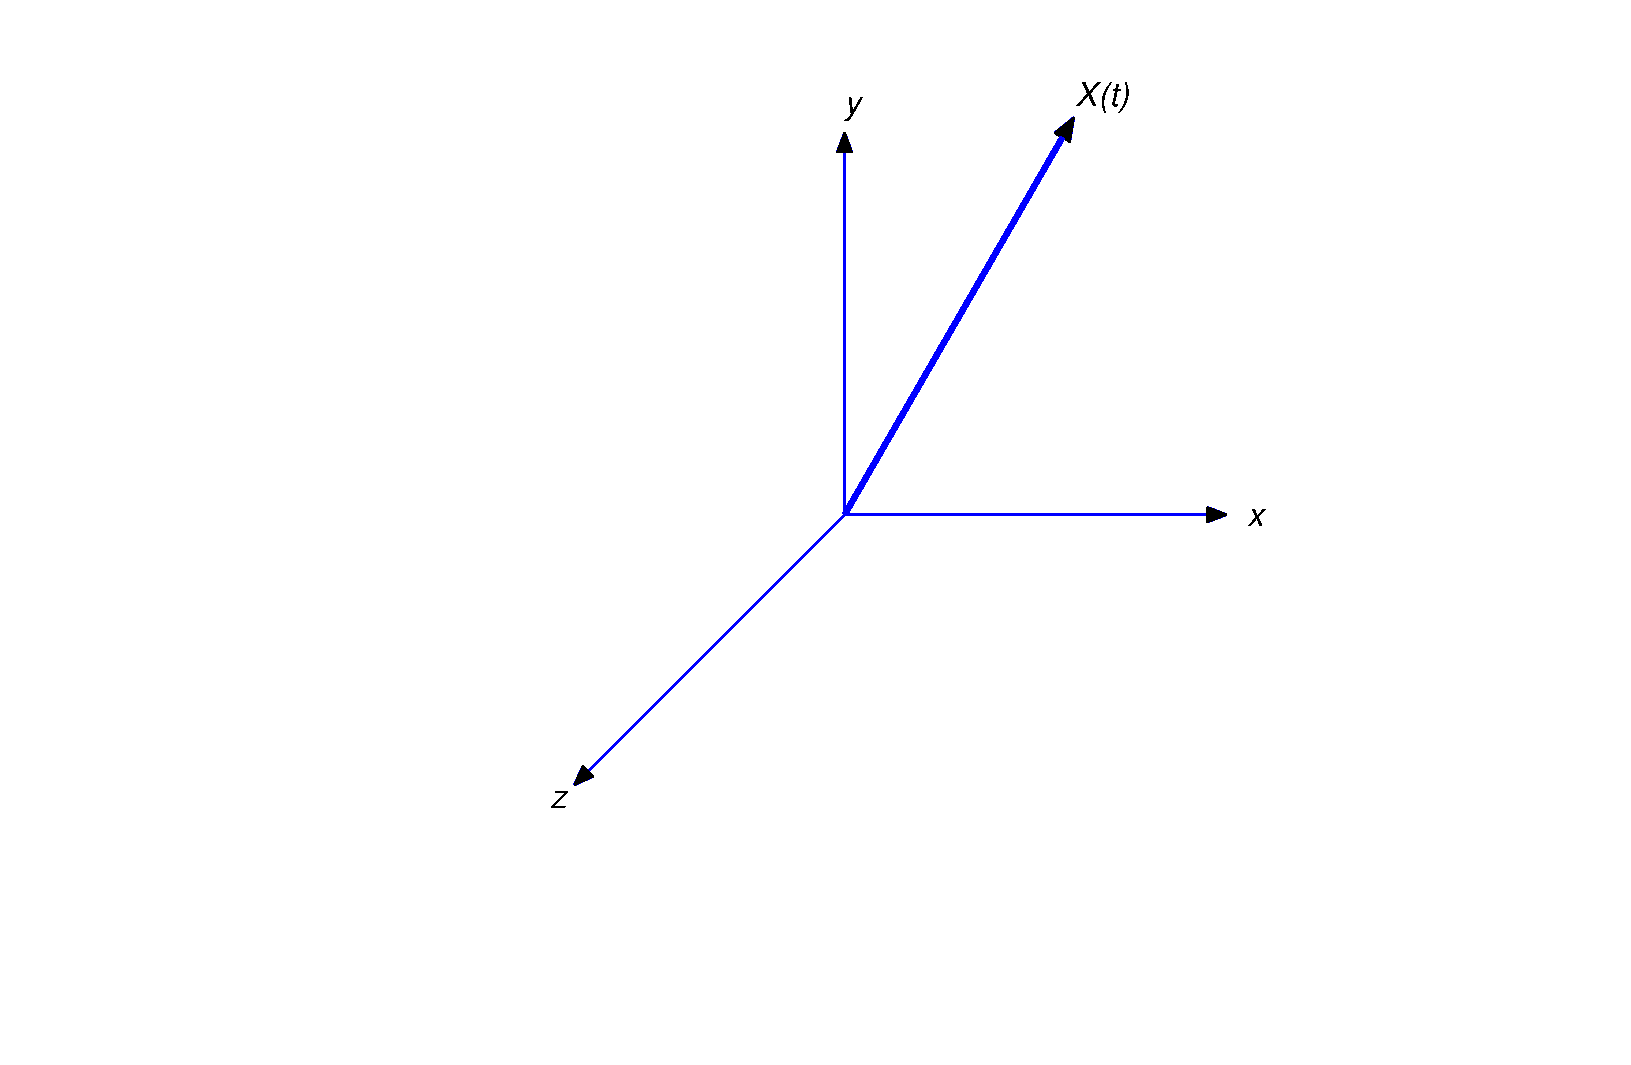
\includegraphics[bb=-78 148 689 643, width=5.67in, height=3.66in, keepaspectratio]{fig100103}
  \caption{}
  \label{figure:10.1.3}
\end{figure}

\boxit{Rewriting Higher Order Systems as First Order Systems}

\noindent
A system of the form
\begin{equation}
  \label{eq:10.1.15}
  \begin{array}{ccl}
    y_{1}' & =      & g_{1}(t,y_{1},y_{2},\dots,y_{n}) \\
    y_{2}' & =      & g_{2}(t,y_{1},y_{2},\dots,y_{n}) \\
           & \vdots &                                  \\
    y_{n}' & =      & g_{n}(t,y_{1},y_{2},\dots,y_{n})
  \end{array}
\end{equation}
is called a {\color{blue}\it first order system\/}, since the only derivatives occurring in it are
first derivatives. The derivative of each of the unknowns may depend upon the independent variable
and all the unknowns, but not on the derivatives of other unknowns. When we wish to emphasize the
number of unknown functions in \eqref{eq:10.1.15} we will say that \eqref{eq:10.1.15} is an
$n\times n$ system.

Systems involving higher order derivatives can often be reformulated as first order systems by
introducing additional unknowns. The next two examples illustrate this.

\begin{example}
  \label{example:10.1.4} \rm Rewrite the system
  \begin{equation}
    \label{eq:10.1.16}
    \begin{array}{rcl}
      m_{1}y_{1}'' & = & -(c_{1}+c_{2})y_{1}'+c_{2}y_{2}'-(k_{1}+k_{2})y_{1}+k_{2}y_{2}+F_{1} \\[1\jot]
      m_{2}y_{2}'' & = & c_{2}y_{1}'-c_{2}y_{2}'+k_{2}y_{1}-k_{2}y_{2}+F_{2}.
    \end{array}
  \end{equation}
  derived in Example~\ref{example:10.1.2} as a system of first order equations.
\end{example}

\solution{} If we define $v_{1}=y_{1}'$ and $v_{2}=y_{2}'$, then $v_{1}'=y_{1}''$ and
$v_{2}'=y_{2}''$, so \eqref{eq:10.1.16} becomes
\[
  \begin{array}{rcl}
    m_{1}v_{1}' & = & -(c_{1}+c_{2})v_{1}+c_{2}v_{2}-(k_{1}+k_{2})y_{1}+k_{2}y_{2}+F_{1} \\[1\jot]
    m_{2}v_{2}' & = & c_{2}v_{1}-c_{2}v_{2}+k_{2}y_{1}-k_{2}y_{2}+F_{2}.
  \end{array}
\]
Therefore $\{y_{1},y_{2},v_{1},v_{2}\}$ satisfies the $4\times4$ first order system
\begin{equation}
  \label{eq:10.1.17}
  \begin{array}{rcl}
    y_{1}' & = & v_{1}                                                                                              \\[1\jot]
    y_{2}' & = & v_{2}                                                                                              \\[1\jot]
    v_{1}' & = & \dst\frac{1}{m_{1}}\left[-(c_{1}+c_{2})v_{1}+c_{2}v_{2}-(k_{1}+k_{2})y_{1}+k_{2}y_{2}+F_{1}\right] \\[1\jot]
    v_{2}' & = & \dst\frac{1}{m_{2}}\left[c_{2}v_{1}-c_{2}v_{2}+k_{2}y_{1}-k_{2}y_{2}+F_{2}\right].
  \end{array}
\end{equation}

\color{blue}
\remark{ The difference in form between \eqref{eq:10.1.15} and \eqref{eq:10.1.17}, due to the way in
which the unknowns are {\color{blue}\it denoted} in the two systems, isn't important;
\eqref{eq:10.1.17} is a first order system, in that each equation in \eqref{eq:10.1.17} expresses
the first derivative of one of the unknown functions in a way that does not involve derivatives of
any of the other unknowns.}
\color{black}

\begin{example}
  \label{example:10.1.5} \rm Rewrite the system
  \[
    \begin{array}{ccc}
      x''  & = & f(t,x,x',y,y',y'') \\[1\jot]
      y''' & = & g(t,x,x',y,y',y'')
    \end{array}
  \]
  as a first order system.
\end{example}

\solution We regard $x$, $x'$, $y$, $y'$, and $y''$ as unknown functions, and rename them
\[
  x=x_{1},\;x'=x_{2},\quad y=y_{1},\quad y'=y_{2},\quad y''=y_{3}.
\]
These unknowns satisfy the system
\[
  \begin{array}{ccl}
    x_{1}' & = & x_{2}                               \\[1\jot]
    x_{2}' & = & f(t,x_{1},x_{2},y_{1},y_{2},y_{3})  \\[1\jot]
    y_{1}' & = & y_{2}                               \\[1\jot]
    y_{2}' & = & y_{3}                               \\[1\jot]
    y_{3}' & = & g(t,x_{1},x_{2},y_{1},y_{2},y_{3}).
  \end{array}
\]

\boxit{Rewriting Scalar Differential Equations as Systems}

\noindent
In this chapter we'll refer to differential equations involving only one unknown function as
{\color{blue}\it scalar\/} differential equations. Scalar differential equations can be rewritten as
systems of first order equations by the method illustrated in the next two examples.

\begin{example}
  \label{example:10.1.6} \rm Rewrite the equation
  \begin{equation}
    \label{eq:10.1.18}y^{(4)}+4y'''+6y''+4y'+y=0
  \end{equation}
  as a $4\times4$ first order system.
\end{example}

\solution We regard $y$, $y'$, $y''$, and $y'''$ as unknowns and rename them
\[
  y=y_{1},\quad y'=y_{2},\quad y''=y_{3},\mbox{\quad and \quad}y'''=y_{4}.
\]
Then $y^{(4)}=y_{4}'$, so \eqref{eq:10.1.18} can be written as
\[
  y_{4}'+4y_{4}+6y_{3}+4y_{2}+y_{1}=0.
\]
Therefore $\{y_{1},y_{2},y_{3},y_{4}\}$ satisfies the system
\begin{eqnarray*}
  y_{1}' & = & y_{2} \\
  y_{2}' & = & y_{3} \\
  y_{3}' & = & y_{4} \\
  y_{4}' & = & -4y_{4}-6y_{3}-4y_{2}-y_{1}.\bbox
\end{eqnarray*}

\begin{example}
  \label{example:10.1.7} \rm Rewrite
  \[
    x'''=f(t,x,x',x'')
  \]
  as a system of first order equations.
\end{example}

\solution We regard $x$, $x'$, and $x''$ as unknowns and rename them
\[
  x=y_{1},\quad x'=y_{2},\mbox{\quad and \quad}x''=y_{3}.
\]
Then
\[
  y_{1}'=x'=y_{2},\quad y_{2}'=x''=y_{3},\mbox{\quad and \quad}y_{3}'=x'''.
\]
Therefore $\{y_{1},y_{2},y_{3}\}$ satisfies the first order system
\[
  \begin{array}{ccl}
    y_{1}' & = & y_{2}                   \\[2\jot]
    y_{2}' & = & y_{3}                   \\[1\jot]
    y_{3}' & = & f(t,y_{1},y_{2},y_{3}).
  \end{array}
\]

Since systems of differential equations involving higher derivatives can be rewritten as first order
systems by the method used in Examples~\ref{example:10.1.5} --\ref{example:10.1.7} , we'll consider
only first order systems.

\boxit{Numerical Solution of Systems}

\noindent
The numerical methods that we studied in Chapter~3 can be extended to systems, and most differential
equation software packages include programs to solve systems of equations. We won't go into detail
on numerical methods for systems; however, for illustrative purposes we'll describe the Runge-Kutta
method for the numerical solution of the initial value problem
\begin{eqnarray*}
  y_{1}' & = & g_{1}(t,y_{1},y_{2}),\quad y_{1}(t_{0})=y_{10}, \\
  y_{2}' & = & g_{2}(t,y_{1},y_{2}),\quad y_{2}(t_{0})=y_{20}
\end{eqnarray*}
at equally spaced points $t_{0}$, $t_{1}$, \dots, $t_{n}=b$ in an interval $[t_{0},b]$. Thus,
\[
  t_{i}=t_{0}+ih,\quad i=0,1,\dots,n,
\]
where
\[
  h=\frac{b-t_{0}}{n}.
\]
We'll denote the approximate values of $y_{1}$ and $y_{2}$ at these points by
$y_{10},y_{11},\dots,y_{1n}$ and $y_{20},y_{21},\dots,y_{2n}$. The Runge-Kutta method computes these
approximate values as follows: given $y_{1i}$ and $y_{2i}$, compute
\begin{eqnarray*}
  I_{1i} & = & g_{1}(t_{i},y_{1i},y_{2i}),                                                            \\
  J_{1i} & = & g_{2}(t_{i},y_{1i},y_{2i}),                                                            \\
  I_{2i} & = & g_{1}\left(t_{i}+\frac{h}{2},y_{1i}+\frac{h}{2}I_{1i},y_{2i}+\frac{h}{2}J_{1i}\right), \\
  J_{2i} & = & g_{2}\left(t_{i}+\frac{h}{2},y_{1i}+\frac{h}{2}I_{1i},y_{2i}+\frac{h}{2}J_{1i}\right), \\
  I_{3i} & = & g_{1}\left(t_{i}+\frac{h}{2},y_{1i}+\frac{h}{2}I_{2i},y_{2i}+\frac{h}{2}J_{2i}\right), \\
  J_{3i} & = & g_{2}\left(t_{i}+\frac{h}{2},y_{1i}+\frac{h}{2}I_{2i},y_{2i}+\frac{h}{2}J_{2i}\right), \\
  I_{4i} & = & g_{1}(t_{i}+h,y_{1i}+hI_{3i},y_{2i}+hJ_{3i}),                                          \\
  J_{4i} & = & g_{2}(t_{i}+h,y_{1i}+hI_{3i},y_{2i}+hJ_{3i}),
\end{eqnarray*}
and
\begin{eqnarray*}
  y_{1,i+1} & = & y_{1i}+\frac{h}{6}(I_{1i}+2I_{2i}+2I_{3i}+I_{4i}), \\
  y_{2,i+1} & = & y_{2i}+\frac{h}{6}(J_{1i}+2J_{2i}+2J_{3i}+J_{4i})
\end{eqnarray*}
for $i=0$, \dots, $n-1$. Under appropriate conditions on $g_{1}$ and $g_{2}$, it can be shown that
the global truncation error for the Runge-Kutta method is $O(h^{4})$, as in the scalar case
considered in Section~3.3.

\exercises

\begin{exerciselist}
  \item\label{exer:10.1.1} Tanks $T_{1}$ and $T_{2}$ contain 50 gallons and 100 gallons of salt
        solutions, respectively. A solution with 2 pounds of salt per gallon is pumped into $T_{1}$
        from an external source at $1$~gal/min, and a solution with $3$ pounds of salt per gallon is
        pumped into $T_{2}$ from an external source at $2$~gal/min. The solution from $T_{1}$ is
        pumped into $T_{2}$ at $3$ gal/min, and the solution from $T_{2}$ is pumped into $T_{1}$ at
        $4$ gal/min. $T_{1}$ is drained at $2$~gal/min and $T_{2}$ is drained at $1$~gal/min. Let
        $Q_{1}(t)$ and $Q_{2}(t)$ be the number of pounds of salt in $T_{1}$ and $T_{2}$,
        respectively, at time $t>0$. Derive a system of differential equations for $Q_{1}$ and
        $Q_{2}$. Assume that both mixtures are well stirred.

  \item\label{exer:10.1.2} Two 500 gallon tanks $T_{1}$ and $T_{2}$ initially contain 100 gallons
        each of salt solution. A solution with $2$ pounds of salt per gallon is pumped into $T_{1}$
        from an external source at $6$~gal/min, and a solution with $1$ pound of salt per gallon is
        pumped into $T_{2}$ from an external source at $5$~gal/min. The solution from $T_{1}$ is
        pumped into $T_{2}$ at $2$ gal/min, and the solution from $T_{2}$ is pumped into $T_{1}$ at
        $1$ gal/min. Both tanks are drained at $3$~gal/min. Let $Q_{1}(t)$ and $Q_{2}(t)$ be the
        number of pounds of salt in $T_{1}$ and $T_{2}$, respectively, at time $t>0$. Derive a
        system of differential equations for $Q_{1}$ and $Q_{2}$ that's valid until a tank is about
        to overflow. Assume that both mixtures are well stirred.

  \item\label{exer:10.1.3} A mass $m_{1}$ is suspended from a rigid support on a spring $S_{1}$ with
        spring constant $k_{1}$ and damping constant $c_{1}$. A second mass $m_{2}$ is suspended
        from the first on a spring $S_{2}$ with spring constant $k_{2}$ and damping constant
        $c_{2}$, and a third mass $m_{3}$ is suspended from the second on a spring $S_{3}$ with
        spring constant $k_{3}$ and damping constant $c_{3}$. Let $y_{1}=y_{1}(t)$,
        $y_{2}=y_{2}(t)$, and $y_{3}=y_{3}(t)$ be the displacements of the three masses from their
        equilibrium positions at time $t$, measured positive upward. Derive a system of differential
        equations for $y_{1}$, $y_{2}$ and $y_{3}$, assuming that the masses of the springs are
        negligible and that vertical external forces $F_{1}$, $F_{2}$, and $F_{3}$ also act on the
        masses.

  \item\label{exer:10.1.4} Let ${\bf X}=x\,{\bf i}+y\,{\bf j}+z\,{\bf k}$ be the position vector of
        an object with mass $m$, expressed in terms of a rectangular coordinate system with origin
        at Earth's center (Figure~\ref{figure:10.1.3}). Derive a system of differential equations
        for $x$, $y$, and $z$, assuming that the object moves under Earth's gravitational force
        (given by Newton's law of gravitation, as in Example~\ref{example:10.1.3} ) and a resistive
        force proportional to the speed of the object. Let $\alpha$ be the constant of
        proportionality.

  \item\label{exer:10.1.5} Rewrite the given system as a first order system.

  \begin{tabular}[t]{@{}p{168pt}@{}p{168pt}}
    ${\bf(a)}\begin{array}{lcc}x'''=f(t,x,y,y')\\[1\jot]y''= g(t,y,y')\end{array}$ & {\bf (b)}$\begin{array}{lcl}u'= f(t,u,v,v',w')\\[1\jot]v''=g(t,u,v,v',w) \\[1\jot]w''=h(t,u,v,v',w,w')\end{array}$ \\[30pt]
    {\bf (c)} $y'''= f(t,y,y',y'')$                                                & {\bf (d)} $y^{(4)}=f(t,y)$                                                                                         \\[20pt]
    {\bf (e)}$\begin{array}{lcc}x''=f(t,x,y)\\[1\jot]y''= g(t,x,y)\end{array}$
  \end{tabular}

  \item\label{exer:10.1.6} Rewrite the system \eqref{eq:10.1.14} of differential equations derived
        in Example~\ref{example:10.1.3} as a first order system.

  \item\label{exer:10.1.7} Formulate a version of Euler's method (Section~3.1) for the numerical
        solution of the initial value problem
  \[
    \begin{array}{rcl}
      y_{1}' & = & g_{1}(t,y_{1},y_{2}),\quad y_{1}(t_{0})=y_{10}, \\
      y_{2}' & = & g_{2}(t,y_{1},y_{2}),\quad y_{2}(t_{0})=y_{20},
    \end{array}
  \]
  on an interval $[t_{0},b]$.

  \item\label{exer:10.1.8} Formulate a version of the improved Euler method (Section~3.2) for the
        numerical solution of the initial value problem
  \[
    \begin{array}{rcl}
      y_{1}' & = & g_{1}(t,y_{1},y_{2}),\quad y_{1}(t_{0})=y_{10}, \\
      y_{2}' & = & g_{2}(t,y_{1},y_{2}),\quad y_{2}(t_{0})=y_{20},
    \end{array}
  \]
  on an interval $[t_{0},b]$.
\end{exerciselist}
